\documentclass[letterpaper, 12pt]{article}
\usepackage[letterpaper, top=2.5cm, bottom=2.5cm, left=3cm, right=3cm]{geometry} %margenes
\usepackage[utf8]{inputenc} %manejo de caracteres especiales
\usepackage[spanish]{babel} %manejo de encabezados de inglés a español
\usepackage{fancyhdr} %formato de los encabezados de página
\usepackage{ragged2e} %alineado real justficado
\usepackage{graphicx} %manejo de imagenes
\usepackage{amsmath} %manejo de notación matemática
\usepackage{mathtools} %manejo de notación matemática
\usepackage{blindtext} %texto de relleno
\usepackage{amssymb} %manejo de simbología variada
\usepackage[backend=biber]{biblatex}\addbibresource{referencias.bib}
\usepackage[titles]{tocloft} %manejo de elementos para el índice
\usepackage{float} %manejo de centrado para figuras
\usepackage{algorithm2e} %manejo de algoritmos
\usepackage{hyperref} %manejo d hipervínculos
\hypersetup{
    colorlinks=true,      
    urlcolor=blue,
    linkcolor=blue
}

\pagestyle{fancy}
\fancyhf{}
\rfoot{\thepage}

\nocite{*}

\makeatletter
\renewcommand*\env@matrix[1][\arraystretch]{%
  \edef\arraystretch{#1}%
  \hskip -\arraycolsep
  \let\@ifnextchar\new@ifnextchar
  \array{*\c@MaxMatrixCols c}}
\makeatother

\begin{document}
    
    %PORTADA
    \begin{titlepage}
        \begin{figure}[ht]
            \centering
            
\includegraphics[width=15cm]{logosITT.png}
        \end{figure}
        \centering
        {\scshape\LARGE Tecnológico Nacional de México\\Instituto Tecnológico de Tijuana\par}
        \vspace{1cm}
        {\scshape\Large Investigación de Operaciones\par}
        \vspace{1cm}
        {\scshape\Large Unidad 3\par}
        \vspace{1.5cm}
        {\huge\bfseries Tema 3.1\\Conceptos básicos de problemas de programación no lineal\par}
        \vspace{2cm}
        {\Large\itshape Equipo No. 1:\\Benites Palacios Jesús Alfredo,\,17212109\\Chino Jimenez Kevin Alejandro,\, 19211616\\Flores Azcona Abraham Jhared,\,19211640\\Nuñez Cano David,\,19211696\\Sanchez Deseusa Victor Manuel,\,19211732\\Sandoval Arce Arath,\,19211734\par}
        \vfill
        Profesora: \par
        Ing. Igreyne Aracely Ruiz Romero
        
        \vfill

        {\large 20 de noviembre del 2020}
    \end{titlepage}

    \newpage
    \thispagestyle{empty}
    \tableofcontents
    \listoffigures

    \newpage
    \lhead{\textbf{Conceptos básicos}}
    \section{Introducción}
    Como se ha visto a lo largo de la asignatura, los tipos de problemas vistos en clase se pueden resolver por planteamientos lineales, pero cuando no se pueden plantear de esa forma, la programación no lineal nos permite resolverlos. Para ello es necesario conocer a grandes rasgos
    los conceptos de dicho paradígma para emplearlos.

    \section{Programación no lineal}
    \subsection{Definición formal}
    \begin{figure}[H]
        \justify
        Permite que \(m,n,p\in\mathbb{Z}\). También que \(X\subset\mathbb{R}^n;\, (f,g_i,h_j):X\rightarrow \mathbb{R} \text{ para cada } i\in \{1,...,m\} \text{ y cada }j\in \{1,...,p\}\) con al menos una \(f,g_i,h_i\) que sea no lineal.
        \\Entonces un problema de optimización no lineal es:
        \[\begin{matrix}
            F.O&\text{min}f(x) \text{ ó max}f(x)&&\\
            \text{S.a:}&g_i(x)\leq 0&\text{para cada }i\in \{1,...,m\}\\
            &h_j=0&\text{ para cada }j\in \{1,...,p\}\\
            &x\in X
        \end{matrix}\]
        \caption{Formalidad del problema de optimización de programación no lineal.}
        \label{fig:formulazo}
    \end{figure}
    \subsection{Definición informal}
    Es el proceso de resolución de un sistema de igualdades y desigualdades sujetas a un conjunto de restricciones sobre un conjunto de variables reales desconocídas, con una función objetivo no son lineales.
    \subsection{Tipos de problemas}
    A grandes rasgos, los problemas de PNL (Programación No Lineal) se pueden clasificar de las siguientes maneras:
    \begin{itemize}
        \item \emph{Optimización sin restricciónes:} la función objetivo no tiene restricciones.
        \item \emph{Programación Lineal: }la función objetivo y sus funciones de restricción son lineales.
        \item \emph{Programación cuadrática: }la función objetivo es cuadrática y sus funciones de restricción son lineales.
        \item \emph{Programación cuadrática cuadráticamente restringida:}la función objetivo y sus funciones de restricción son cuadráticas.
        \item \emph{Programación cónica de 2do. órden: }la función objetivo es lineal y se minimiza sobre la intersección de un conjunto afín y del producto de conos de segundo órden.
        \item \emph{Programación semidefinidad:}la función objetivo es es minimizada sujeta a una desigualda de una matríz lineal.
    \end{itemize}
    Un caso especial de los problemas de PNL es la \emph{programación convexa} en la cual todas las soluciones locales son soluciones globales.
    \subsection{Dificultades del paradígma}
    \begin{itemize}
        \item La solución óptima no siempre se encuentra en un punto extremo de la región factible.
        \item Hay casos donde el punto óptimo está en el interior de la región factible.
        \item Generalmente \emph{se encuentra un óptimo local ó relativo, mas nó el óptimo global ó absoluto.}
        \item La función objetivo, las restricciones ó ambas puedem ser no lineales.
        \item Se pueden generar regiones de factibilidad que no son necesariamente convexas.
    \end{itemize}
    \subsubsection{Distinción entre un máx/min local y global}
    Debido a las restricciones que se impongan y el comportamiento mismo de la función objetivo generan un incoveniente donde las soluciones ante el problema no son las soluciones más efectivas.
    \begin{figure}[H]
        \centering
        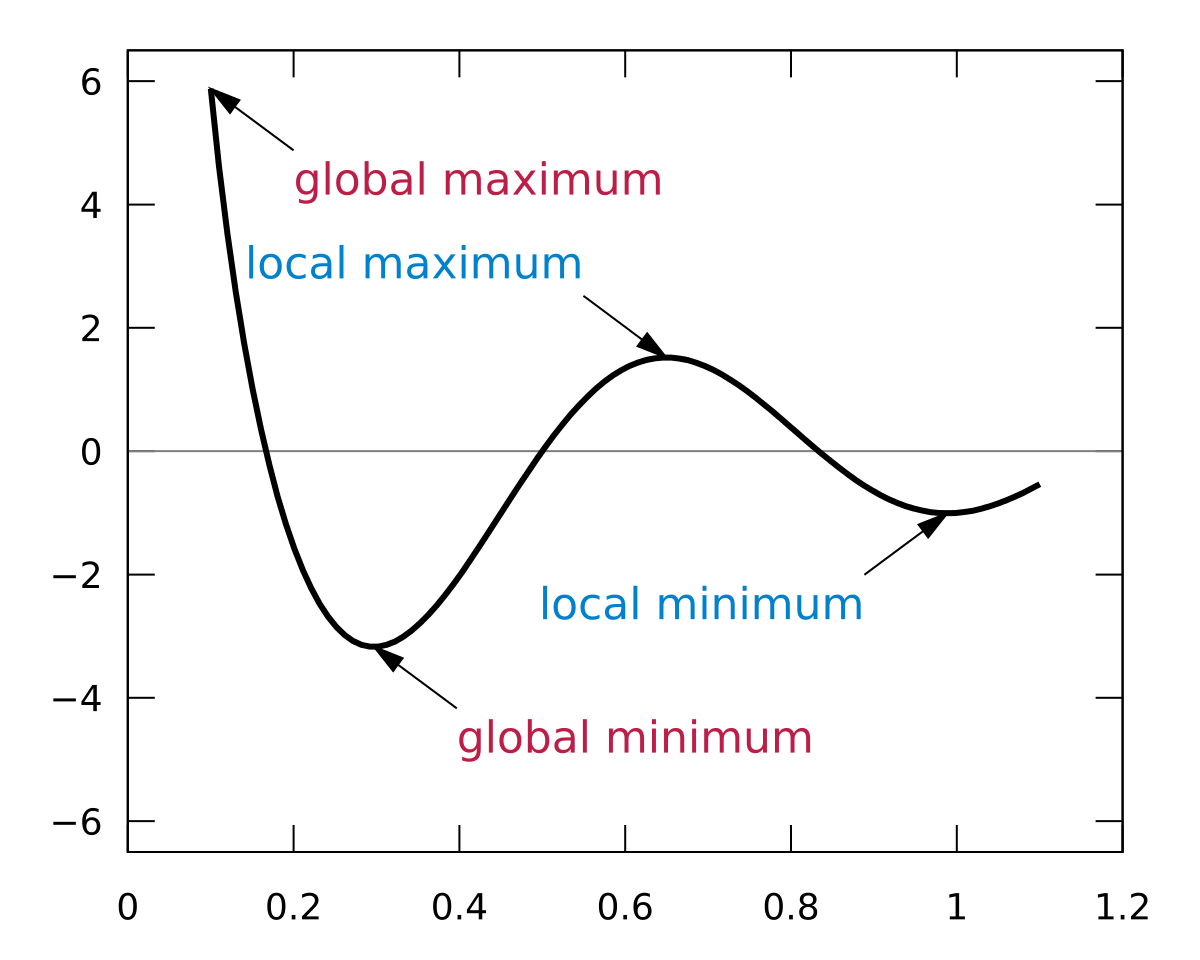
\includegraphics[width=8cm]{ejemplomaxmins.png}
        \caption{Ejemplo de máximos y mínimos locales y globales dada una función \(f(x)\).}
        \label{fig:maxmins}
    \end{figure}
    \justify
    Como se aprecia en la imágen \ref{fig:maxmins}, si se resolviese un problema de optimización no lineal las posibles soluciones pueden no ser las ``verdaderas soluciones'' que pudiesen alcanzarse.
    Una razón de esto es la restricción de valores para la misma función, lo que nos límita a solamente ciertos valores, los cuales pueden contener ó no un máximo o mínimo global.
    \subsection{Ejemplo: Optimización unidimensional no restringida por \emph{Criterio de la Segunda Derivada}}
    Uno de los acercamientos previos a este tipo de optimización se explicó en la materia de Cálculo Diferencial como \emph{Criterio de la Segunda Derivada}, el cuál permite conocer los máximos o mínimos locales de
    una función de una sola variable. \\\newline Consideramos que dicho procedimiento es amigable para comprender a grandes rasgos la noción de la NPL debido a nuestra exposición y estudio anterior como parte de la asigniatura dicha.
    \subsubsection{Definición}
    \begin{figure}[H]
    \justify
    Admitamos que la función \(y=f(x)\) es continua en el intervalo \((a,b)\) y que \(f'(c)=0\) para algún número \(c\in (a,b)\).\\
    \begin{itemize}
        \item \(f''(c)>0\rightarrow f(c)\) es un \emph{mínimo local de} \(f\).
        \item \(f''(c)<0\rightarrow f(c)\) es un \emph{máximo local de} \(f\).
        \item \(f''(c)=0\rightarrow f(c)\) la prueba es inconclusa para \(f\) y se debe de aplicar el \emph{Críterio de la Primer Derivada}.
    \end{itemize}
    \caption{Formalismo del Criterio de la Segunda Derivada.}
    \label{fig:criterio}
    \end{figure}
    \subsubsection{Práctica}
    Obtener el máximo y mínimo local de la función \(f(x)=\frac{1}{3}x^3-2x^2+3x+1\) por el criterio de la segunda derivada.
    \\\newline\textbf{Pasos: }\\\newline
    \emph{1. Obtener la derivada de \(f(x)\)}.
    \[\begin{matrix}[1.5]
        f'(x)&=&\frac{d}{dx}\left(\frac{1}{3}x^3-2x^2+3x+1\right)\\
        &=&\frac{1}{3}(3)x^{2-1}-(2)(2)x^{2-1}+3\\
        &=&x^2-4x+3
    \end{matrix}\]
    \emph{2. Obtener las raíces de \(f'(x)\)}.
    \[\begin{matrix}
        x^2-4x+3&=&0\\
        (x-3)(x-1)&=&0\therefore\\
        \therefore x-3=0&\text{y}&x-1=0\\
        x=3&\text{y}&x=1
    \end{matrix}\]
    \emph{3. Determinar la segunda derivada de \(f(x)\)}.
    \[\begin{matrix}[1.5]
        f''(x)&=&\frac{d}{dx}f'(x)\\
            &=&\frac{d}{dx}(x^2-4x+3)\\
            &=&2x-4
    \end{matrix}\]
    \emph{4. Evaluar \(f''(3)\) y \(f''(1)\).}
    Para \(f''(3)\):
    \[\begin{matrix}
        f''(3)&=&2(3)-4\\
        &=&6-4\\
        &=&2
    \end{matrix}\]
    Como \(f''(3)>0\) entonces en \(x=3\) la función \emph{admite un mínimo local.} Ahora para \(f''(1)\):
    \[\begin{matrix}
        f''(1)&=&2(1)-4\\
            &=&2-4\\
            &=&-2
    \end{matrix}\]
    Como \(f''(1)<0\) entonces en \(x=1\) la función \emph{admite un máximo local.}
    \\\newline
    \emph{5. Evaluar \(f(x)\) en \(x=1\) y en \(x=3\) para obtener los extremos locales.}
    \[\begin{matrix}[1.5]
        \text{Máximo local}&=&f(1)&=&\frac{1}{3}(1)^3-2(1)^2+3(1)+1&=&\frac{7}{3}\\
        \text{Mínimo locar}&=&f(3)&=&\frac{1}{3}(3)^3-2(3)^2+3(3)+1&=&1
    \end{matrix}\]
    Por lo tanto el máximo local se ubica en \((1,\frac{7}{3})\) y el mínimo local se encuentra en \((3,1)\), lo cual podemos comprobar con la gráfica de \(f(x)\) que se muestra a continuación:
    \begin{figure}[H]
        \centering
        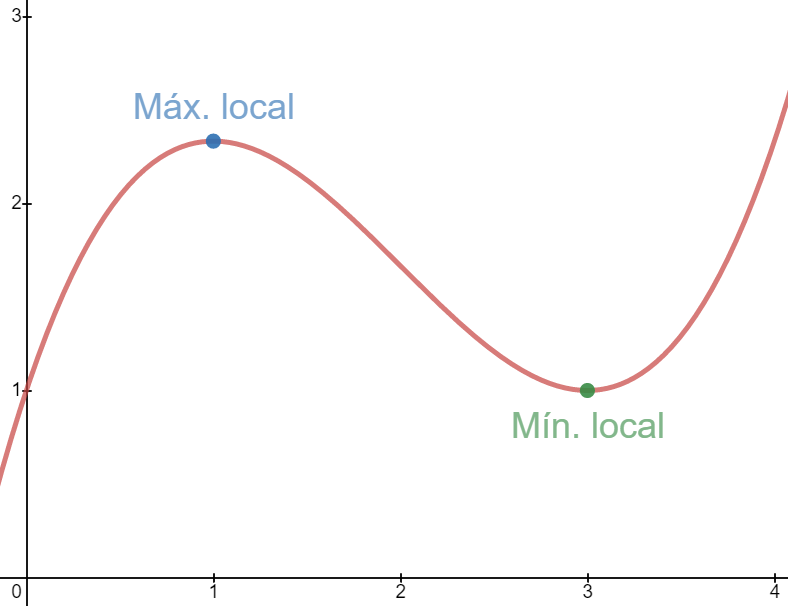
\includegraphics[width=10cm]{fxmaxmin.PNG}
        \caption{Máximos y mínimos locales de \(f(x)\).}
    \end{figure}
    \subsection{Aplicaciones}
    Algunas aplicaciones son las siguientes:
    \begin{itemize}
        \item Optimización de redes neuronales.
        \item Exhibir economías de escala.
        \item Análisis de datos no lineales.
    \end{itemize}
    \subsubsection*{Diapositivas del tema}
    Enlace para ver las diapositivas del tema en Miro: \url{https://miro.com/app/board/o9J_lf0cm0M=/}

    \section{Conclusión}
    La programación no lineal es una de las herramientas mas complejas pero más potentes para los problemas de optimización que se nos interponga, por ello su estudio y compresión
    de sus conceptos básicos nos brinda una mejór base para desarrollar el tema de una manera más elaborada.

    \newpage
    \lhead{}
    \addcontentsline{toc}{section}{Referencias}
    \printbibliography
    \section*{Diapositivas del tema}
    \addcontentsline{toc}{section}{Diapositivas}
    \justify
    \begin{itemize}
        \item \textbf{Enlace para las diapositivas (Miro):} \url{https://miro.com/app/board/o9J_lf0cm0M=/}
    \end{itemize}
    
\end{document}